\section{Lecture 2}

\subsection{Transport through membranes}
\begin{longtable}{p{4cm}p{15cm}}
Cellular membrane	& 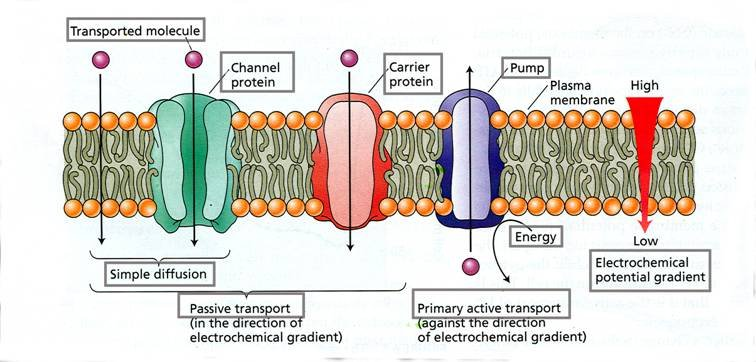
\includegraphics[width = 14cm]{neuroinf_membrane.jpg}\\
Phospholipids		& The membrane consists of a bilayer of phospholipids. The heads are charged and hydrophil. The tails are oily and hydrophob.\\
Passive transport	&\\
- Simple diffusion	& Small, lipophile and non-polar molecules can diffuse through the membrane. They are governed by differnces in concentration and / or charge.\\
- Channel protein	& Within the membrane, there are channels (channel proteins) which have aminoacids at their interior. Therefore, small polar or charged particles like ions can get transported through these channels. Typically, the channels need to be opened chemically, electrically or mechanically.\\
- Carrier protein	& A special carrier protein binds with a certain molecule. The carrier protein changes its conformation at binding. That way, the molecule gets carried through the membrane. There are carrier proteins which can only one or two molecules at once.\\
Active transport	&\\
- Sodium-Potassium Pump	& \begin{itemize}
                       	  	\item The Sodium-Potassium-ATPase (3 Na$^+$ / 2 K$^+$ - ATPase) aka Sodium-Potassium pump is transport protein in the membrane.
				\item The pump is opened at the inside. Three Na$^+$ are taken into the pump.
				\item The pump changes its conformation which leads to the release of Na$^+$ ions to the extracellular fluid. The processes which lead to the conformation need energy, which is yielded by the ATP.
				\item From the ECF, two K$^+$ kations are taken into the pump. Again, a conformational change is invoked and the two K$^+$ are expelled into the ICF.
				\item Per cycle, the pump removes one charge unit from the ICF. Thereby it helps maintaining a resting potential.
                       	  \end{itemize}\\
Typical ion concentrations in body		& \begin{tabular}{lll}
			    Ion		& Interior (mM)	& Exterior(mM)\\\hline
			    Na$^+$	& 15		& 150\\
			    K$^+$	& 150		& 5\\
			    Ca$^{2+}$	& 0		& 2.5\\
			    Cl$^-$	& 110		& 10\\
		\textbf{large Anions}	& \textbf{65}	& \textbf{2}
			  \end{tabular}\\
Gibbs-Donnan-Equilibrium	& Large Anions cannot be transported through the membrane by any means. Also, some ions (potassium) might have a bigger permability. This influences the diffusion of the other ions. Both ICF and ECF must be electrically neutral. At equilibrium, the concentrations of the inner and outer ions are therefore not equal. As a consequence, a persistent potential difference arises.\\
Cellular membrane	& 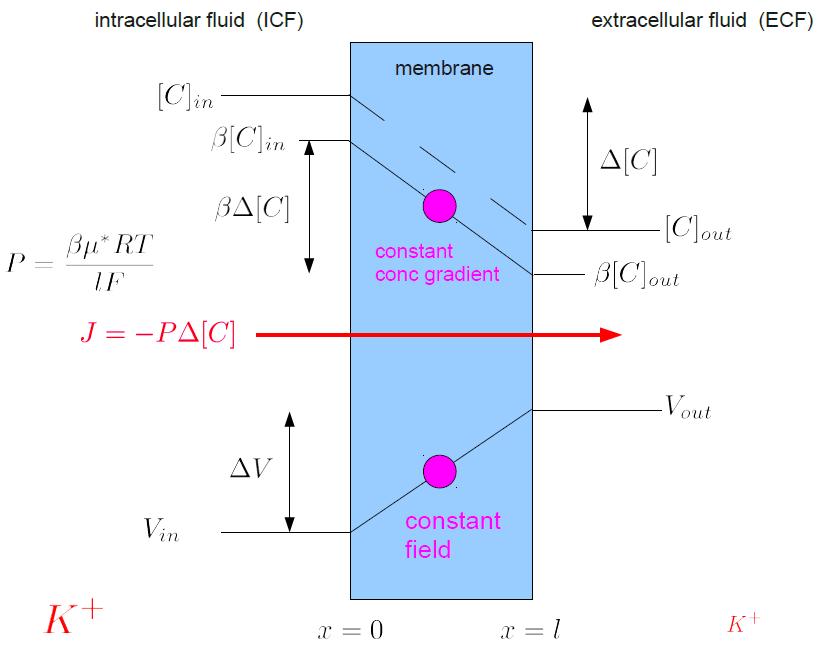
\includegraphics[width = 14cm]{neuroinf_cell_membrane_transport.png}\\
\end{longtable}
\subsection{Maths}
\begin{tabular}{p{4cm}p{15cm}}
Fick's law of diffusion		& \begin{tabular}[t]{l}
				    $\boxed{J_{diff} = -D \frac{ \partial [C]}{\partial x}}$\\
				    $J_{diff}:$ diffusion flux $[$molecules$ / (s \cdot cm^2)]$\\
				    $D:$ diffusion coefficient $[cm^2/s]$\\
				    $[C]:$ concentration of species $[molecules/cm^3]$
				  \end{tabular}\\
Ohm's law of drift		& \begin{tabular}[t]{l}
				    $\boxed{J_{drift} = \partial_{el} E = -\mu z [C] \frac{\partial V}{\partial x}}$\\
				    $J_{drift}:$ drift flux $[$molecules$ / (s \cdot cm^2)]$\\
				    $\partial_{el}$: electrical conductivity $[$molecules$ / (V \cdot s \cdot cm)]$\\
				    $E = -\partial V / \partial x$: electric field $[V/cm]$\\
				    $V:$ electric potential\\
				    $\mu:$ mobility $[cm^2 / (V \cdot s)]$\\
				    $z:$ valence of ion
				  \end{tabular}\\
Einstein Relation		& \begin{tabular}[t]{l}
				    $\boxed{D = \frac{k_B T}{q} \mu = \frac{RT}{F} \mu}$\\
				    $q: $ charge of the molecule [Coulombs]
				  \end{tabular}\\
Nernst-Planck-Equation		& $\boxed{I = J_{tot} \cdot zF = -\left(\mu z^2 F[C] \frac{\partial V}{\partial x} + \mu z RT \frac{\partial [C]}{\partial x}\right)}$\\
Nernst-Equation			& \begin{tabular}[t]{l}
				    Resting potential: Use NPE with no net flux $\Rightarrow I = 0$\\
				    $V_2 - V_1 = -\frac{RT}{zF} \ln \frac{[C]_2}{[C]_1}$\\
				    $\boxed{V_2-V_1 = -\frac{RT}{F} \ln \frac{[C]_{in}}{[C]_{out}}}\quad$ for $ z=1$
				  \end{tabular}\\
				& With the Nernst-equation, we can calculate the voltage difference arising by the Donnan-Equilibrium (aka the resting potential).\\
Prefactor			& $\boxed{\frac{RT}{F} = 26.7 $mV at T $= 37^{\circ}$C$}$ To be used with the natural logarithm (Nernst-equation)\\
				& $\boxed{\frac{RT}{F} \ln(10) = 61.5 $mV at T $= 37^{\circ}$C$}$ To be used with the base 10 logarithm (GHK equation)\\
Permeability			& \begin{tabular}[t]{l}
            			  	$P = \frac{\beta D}{l}$\\
					$\beta$: Water-membrane partition coefficient for ion $i$\\
					$l$: Thickness of membrane.\\
					$J = -P \Delta[C]$
            			  \end{tabular}\\
Goldman-Hodgkin-Katz Equation	& \begin{tabular}[t]{l}
				    $\boxed{\Delta V  = \frac{RT}{F}\cdot\log_{10}\frac{P_{\text{Na}}\cdot[\text{Na}^+]_a+P_\text{K}\cdot[\text{K}^+]_a+P_\text{Cl}\cdot[\text{Cl}^-]_i}
{P_\text{Na}\cdot[\text{Na}^+]_i+P_\text{K}\cdot[\text{K}^+]_i+P_{\text{Cl}}\cdot[\text{Cl}^-]_a}}$\\
				    P = Permeability, $\sum P_i = 1$\\
				    $\Delta V$ is the voltage difference between the interior and the exterior of a cell.
				  \end{tabular}\\
				& The GHK voltage equation is a generalization of the Nernst-equation.
\end{tabular}